\documentclass{article}

\usepackage{graphicx}
\usepackage{tikz}
\usepackage{tikzsymbols}
\usetikzlibrary{calc,patterns,shapes.geometric}
\pagestyle{empty}
\usepackage[margin=0pt]{geometry}
\geometry{papersize={14in,12in}}

\def\centerarc[#1](#2)(#3:#4:#5){\draw[#1] ($(#2)+({#5*cos(#3)},{#5*sin(#3)})$) arc (#3:#4:#5);}

\begin{document}
	\begin{figure}
		\centering
		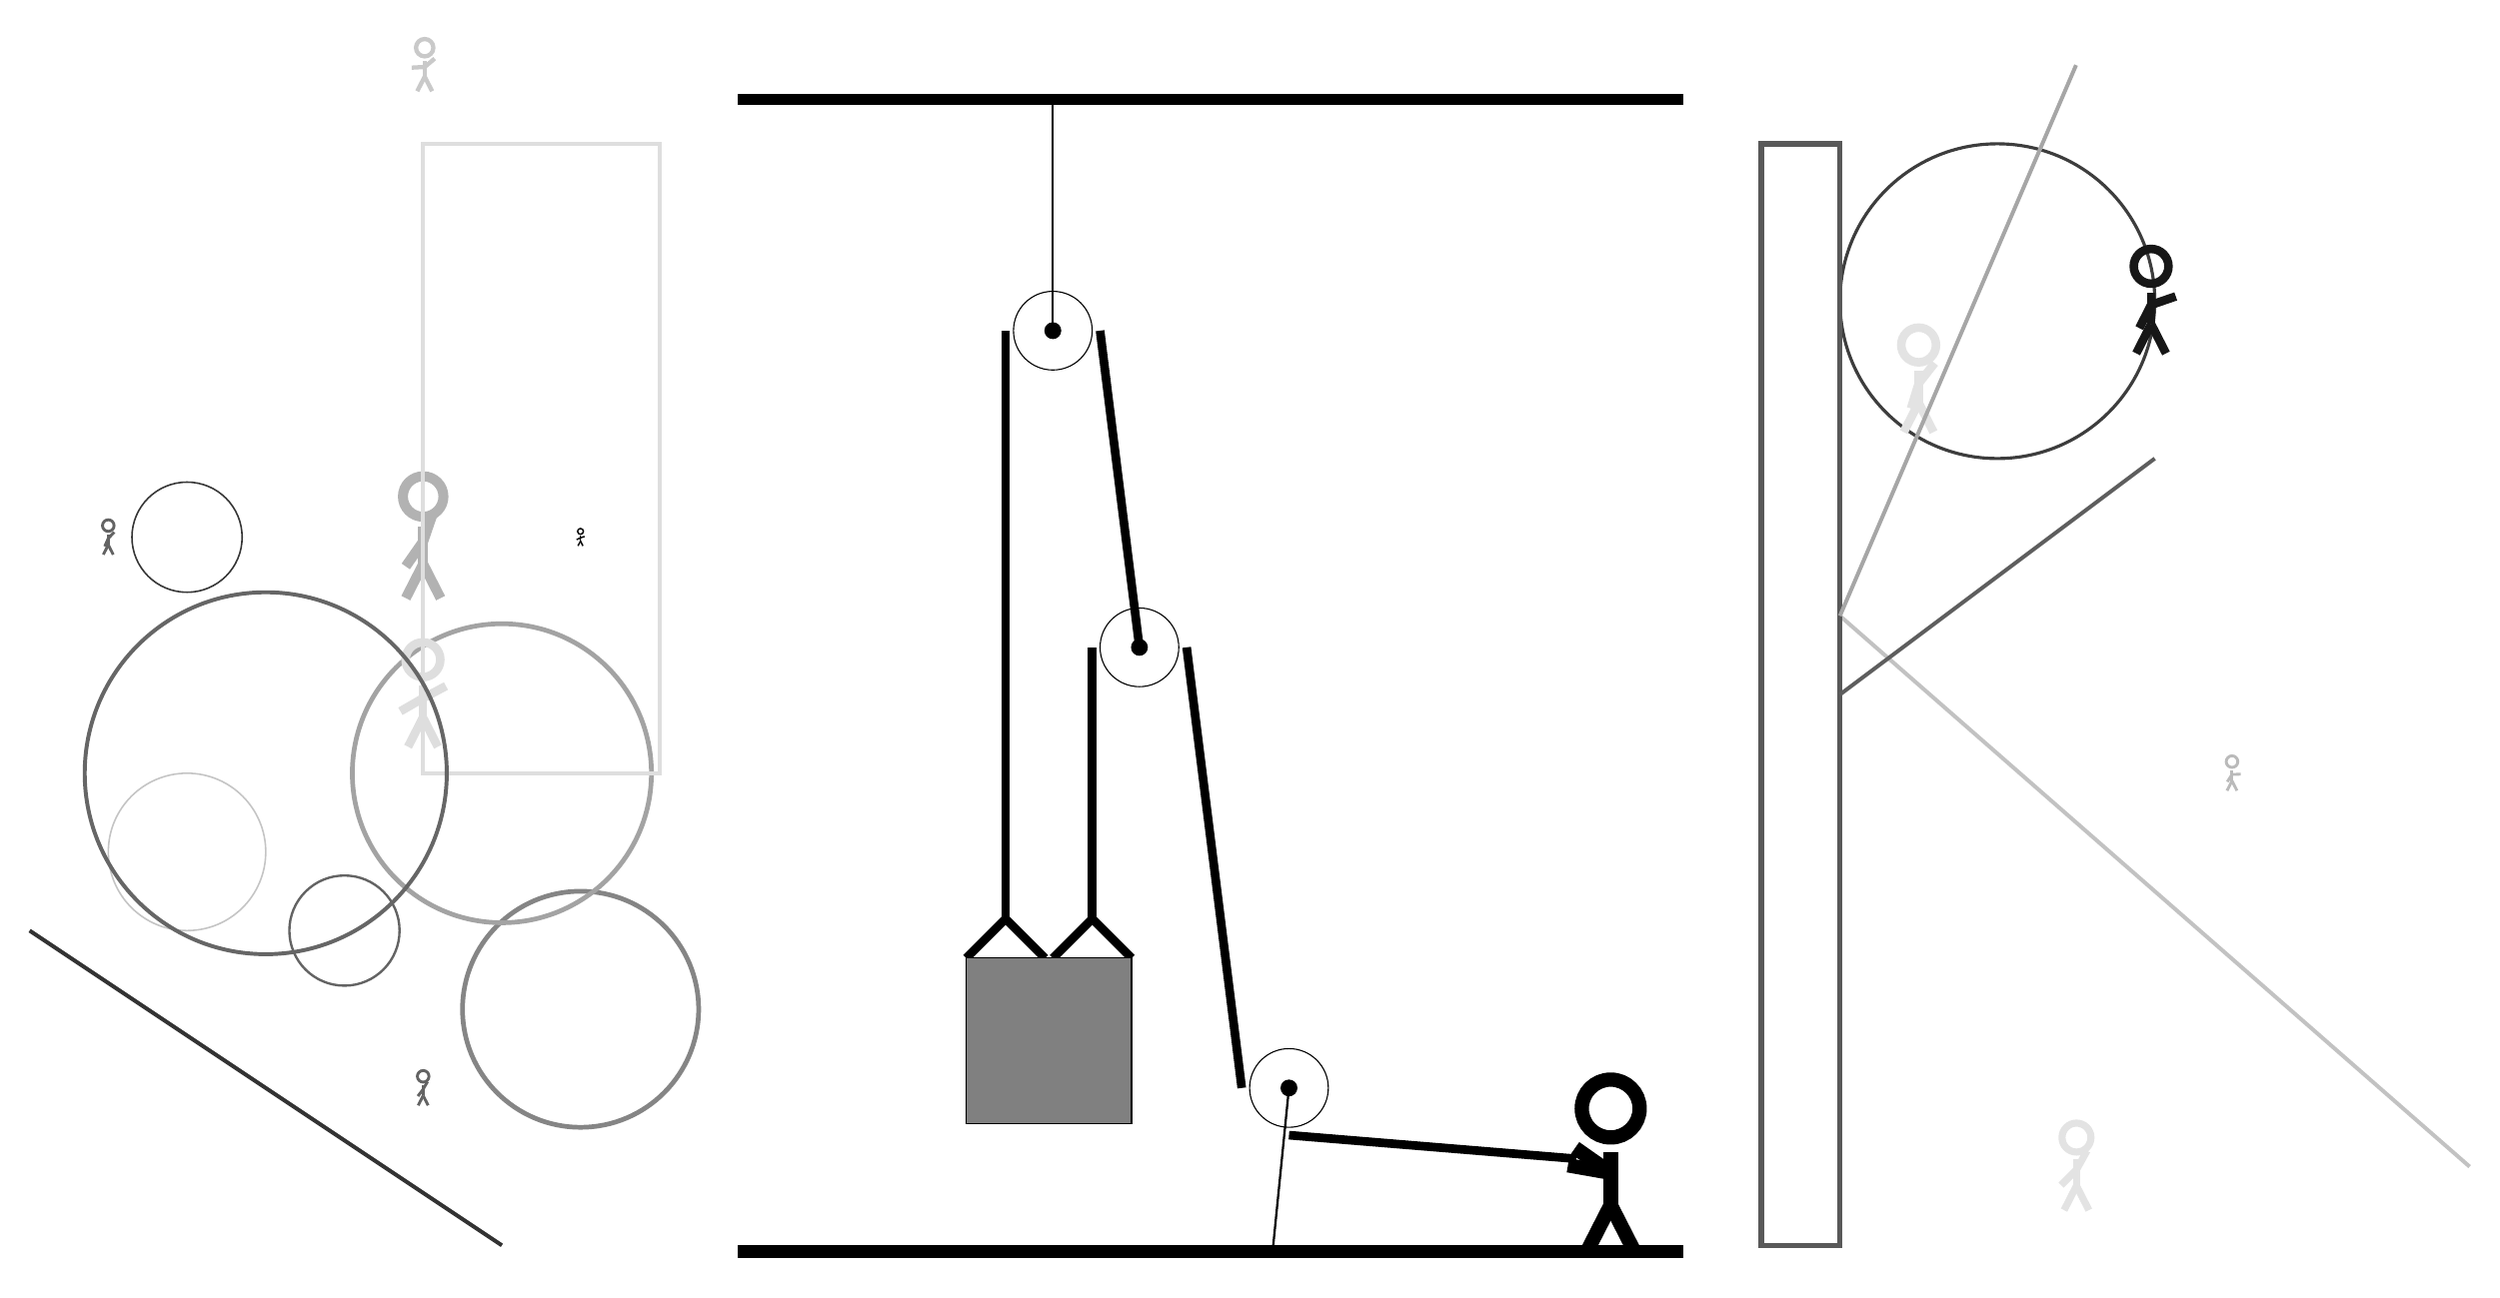
\begin{tikzpicture}
			%%%%% START %%%%%
			
			\draw[fill=black] (-2, 11.5) rectangle (10, 11.625);
			
			\draw (2, 8.625) circle (0.5);
			\draw[fill=black] (2, 8.625) circle (0.1);
			\draw[thick] (2, 8.625) -- (2, 11.5);
			
			\draw (3.1, 4.6) circle (0.5);
			\draw[fill=black] (3.1, 4.6) circle (0.1);
			
			\draw [line width=0.6mm, color=black!48](-4, 0) circle (1.5);
			
			\draw [line width=0.6mm, color=black!36](-5, 3) circle (1.9);
			\draw[line width=0.5mm, color=black!24](12, 5) -- (20, -2);
			\node[line width=0.7mm, color=black!99] at (-4, 6) {\Strichmaxerl[1][25][18]};
			\draw [line width=0.2mm, color=black!79](-9, 6) circle (0.7);
			\node[line width=0.7mm, color=black!13] at (-6, 4) {\Strichmaxerl[6][30][28]};
			
			\node[line width=0.5mm, color=black!27] at (17, 3) {\Strichmaxerl[2][57][2]};
			\draw [line width=0.3mm, color=black!61](-7, 1) circle (0.7);
			\draw [line width=0.4mm, color=black!76](14, 9) circle (2.0);
			
			\draw[line width=0.7mm, color=black!65] (12, -3) rectangle (11, 11);
			\node[line width=0.7mm, color=black!30] at (-6, 6) {\Strichmaxerl[7][55][71]};
			
			\node[line width=0.2mm, color=black!11] at (15, -2) {\Strichmaxerl[5][45][61]};
			\draw [line width=0.2mm, color=black!23](-9, 2) circle (1.0);
			
			\draw[line width=0.5mm, color=black!63](12, 4) -- (16, 7);
			\node[line width=0.5mm, color=black!61] at (-10, 6) {\Strichmaxerl[2][66][47]};
			\node[line width=0.4mm, color=black!61] at (-6, -1) {\Strichmaxerl[2][53][60]};
			\node[line width=0.3mm, color=black!21] at (-6, 12) {\Strichmaxerl[3][3][40]};
			\node[line width=0.5mm, color=black!91] at (16, 9) {\Strichmaxerl[6][63][19]};
			\node[line width=0.5mm, color=black!11] at (13, 8) {\Strichmaxerl[6][73][52]};
			\draw[line width=0.5mm, color=black!35](15, 12) -- (12, 5);
			\draw[line width=0.5mm, color=black!80](-5, -3) -- (-11, 1);
			
			\draw[line width=0.5mm, color=black!13] (-3, 3) rectangle (-6, 11);
			
			\draw [line width=0.5mm, color=black!60](-8, 3) circle (2.3);
			
			\draw (5, -1) circle (0.5);
			\draw[fill=black] (5, -1) circle (0.1);
			\draw[thick] (5, -1) -- (4.8, -3);
			
			\draw[line width = 1.1mm]  (0.9, 0.65) -- (1.4, 1.15) -- (1.9, 0.65);
			\draw[line width = 1.1mm]  (2.0, 0.65) -- (2.5, 1.15) -- (3.0, 0.65);
			\draw[fill=black!50] (0.9, 0.65) rectangle (3.0, -1.45);
			
			\draw[line width = 1.1mm] (1.4, 8.625) -- (1.4, 1.15);
			\centerarc[line width = 1.1mm](2, 8.625)(0:180:0.6);
			\draw[line width = 1.1mm] (2.6, 8.625) -- (3.1, 4.6);
			\draw[line width = 1.1mm] (2.5, 4.6) -- (2.5, 1.15);
			\centerarc[line width = 1.1mm](3.1, 4.6)(0:180:0.6);
			\draw[line width = 1.1mm] (3.7, 4.6) -- (4.4, -1);
			\centerarc[line width = 1.1mm](5, -1)(180:270:0.6);
			\draw[line width = 1.1mm] (5, -1.6) -- (8.65, -1.9);
			
			\node at (9, -2) {\Strichmaxerl[10][-35][170]};
			
			\draw[fill=black] (-2, -3) rectangle (10, -3.15);
			
			%%%%% END %%%%%
		\end{tikzpicture}
	\end{figure}	
\end{document}